\begin{figure}[H]
	\centering
	\begin{tikzpicture}[shorten >=1pt,node distance=2cm,on grid,auto]
		\node[state] (0) {peer-0};
		\node[state] (1) [right=of 0]{peer-1};
		\node[state] (2) [below=of 0]{peer-2};
		\node[state] (3) [right=of 2]{peer-3};
		\path[->]
			(0) edge node {} (1)
			(0) edge node {} (2)
			(0) edge node {} (3)
			
			(1) edge node {} (0)
			(1) edge node {} (2)
			(1) edge node {} (3)
			
			
			(2) edge node {} (0)
			(2) edge node {} (1)
			(2) edge node {} (3)
			
			
			(3) edge node {} (0)
			(3) edge node {} (1)
			(3) edge node {} (2);
	\end{tikzpicture}
	\caption{Raft Cluster Topology}
\end{figure}
In order to test the performance, the researchers organized a 4-node cluster for testing as figure 7. In additional to performance benchmarking, the researchers first applied a fault tolerance testing to validate leader-election by taking down a node in the cluster to see if the Pub/Sub system could still function. In most of the cases, leader nodes are taken down in order to observe how the cluster would re-elect a leader. All experiments suggests the leader re-elections were successful although some may cause significant latency during the process. Once the fault tolerance is confirmed to be successful, the researchers proceeded with performance benchmark.

	
\begin{figure}[H]
	\centering
	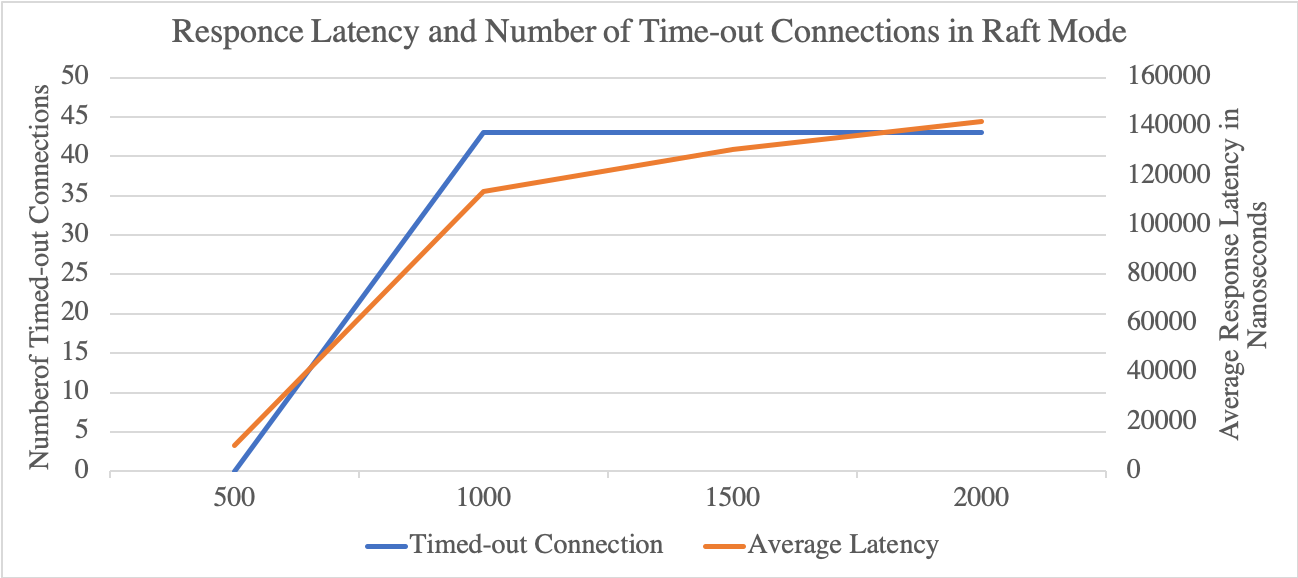
\includegraphics[scale=0.33]{figure/raft/performance.png}
	\caption{Raft Performance}
\end{figure}
	
\begin{figure}[H]
	\centering
	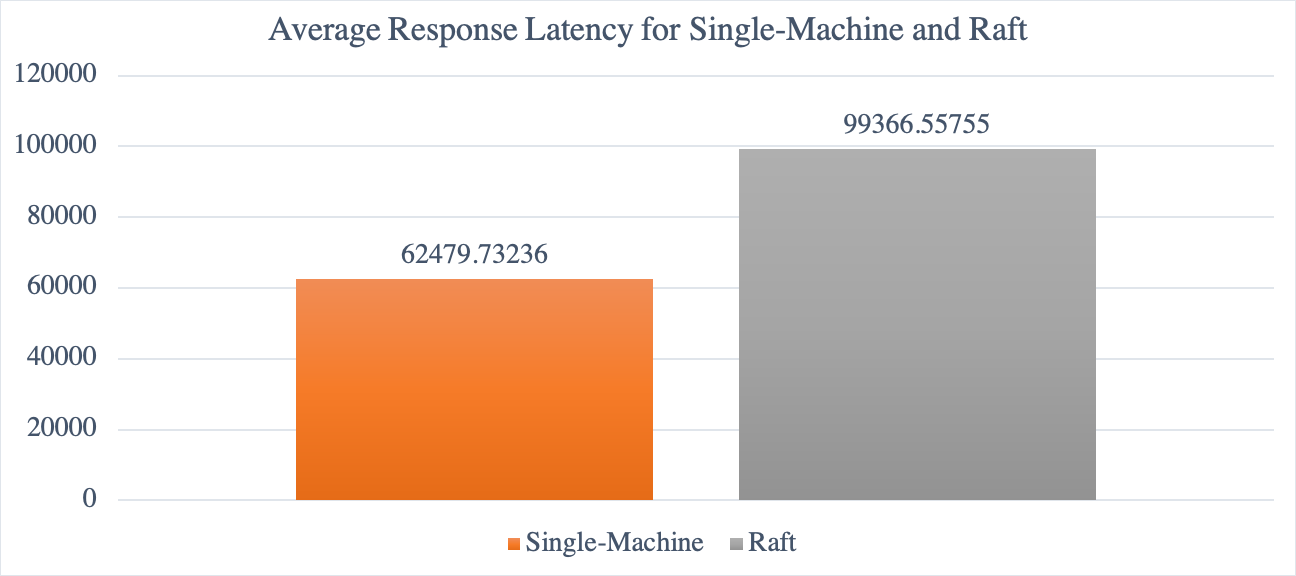
\includegraphics[scale=0.33]{figure/raft/response-latency.png}
	\caption{Single-Machine/Raft average response latency}
\end{figure}

Same in master-slave mode, the clients were evenly distributed onto each node in the cluster. However while testing, the researchers found that the system would be frequently stalled due to Raft-related heartbeat and synchronization operations, if the size of test increment were small. This effect can be cancelled out by extending heartbeat interval, but doing so would make the system behaving more like master-slave mode. Overall, the researchers decided to resolve the issue by increasing the test sample size in aim to reduce the total number of test iterations and internal leader elections. 

As the graph has shown, capacity-wise Raft-mode is still capable of hosting large number of clients. However, the average latency is over 50\% slower than that of a single machine, and timeout rate had also hiked.